\section{Durchführung}
\label{sec:Durchführung}

In \autoref{fig:schema} wird die Messapparatur schematisch dargestellt.
\begin{figure}
    \centering
    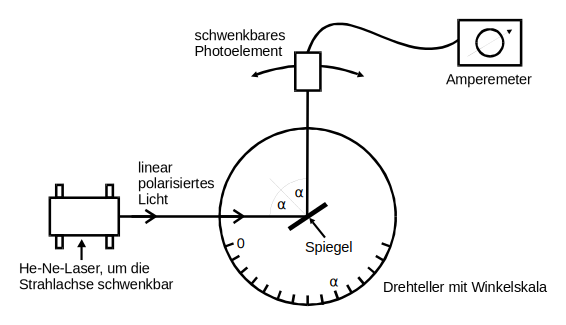
\includegraphics[width=0.8\linewidth]{pictures/schema.pdf}
    \caption{Reflexion und Brechung des parallel polarisierten Lichtstrahls. \cite{v407}}
    \label{fig:schema}
\end{figure}

Durch ein schwenkbares Photoelement wird dabei die Intensität des Lasers gemessen,
welche als Strahlung von einer Si-Oberfläche reflektiert wird.
Um polarisiertes Licht herzustellen, wird ein Polfilter zwischen Laser und Si-Oberfläche platziert.
Zum Einstellen des Einfallswinkels, befindet sich die Si-Oberfläche auf einer Drehscheibe.
Dabei muss darauf geachtet werden, dass der reflektierte Lichtstrahl auf einer festen Höhe der Drehscheibe
die Öffnung des Photoelements fällt.
Durch ein Amperemeter wird der Strom gemessen, der durch das einfallende Licht erzeugt wird.
Nach der Messung des Nullstroms, werden bei einer Schrittweite von $\ang{2;;}$ im Bereich von $\ang{6;;}$ 
bis $\ang{88;;}$ die Ströme jeweils für senkrechte und parallele Polarisation aufgenommen.